% 01_background.tex
\section{The expanding background}
\label{ch:background}

Cosmology is built on a single observational fact -- the universe is homogeneous and isotropic on large scales -- and on a theory that says how spacetime responds to its energy content -- general relativity. From these two ingredients we will derive the Friedmann equation, the equation that controls the expansion rate $H(t)$ of a smooth, expanding universe. We will derive it twice, first by a Newtonian argument and then properly from the Einstein equations, code both up, and use the result to plot the expansion history of our universe. Every later chapter sits on top of what we build here.

\subsection{The FRW metric}

The assumption of homogeneity and isotropy uniquely fixes the spacetime metric, up to an overall time-dependent scale factor $a(t)$ and a curvature parameter $K \in \{-1, 0, +1\}$. The result is the Friedmann-Robertson-Walker (FRW) metric. In the flat case ($K = 0$), which is what Planck observations select to high accuracy, the line element in cosmic time $t$ is
\begin{equation}
  \mathrm{d}s^2 = -\mathrm{d}t^2 + a^2(t)\,\bigl(\mathrm{d}x^2 + \mathrm{d}y^2 + \mathrm{d}z^2\bigr).
  \label{eq:FRW_cosmic}
\end{equation}
The coordinates $(x, y, z)$ are \emph{comoving}: a galaxy that has no peculiar motion stays at fixed $(x, y, z)$ as the universe expands. The physical distance between two such galaxies is $a(t)$ times their coordinate separation. The function $a(t)$ -- the scale factor -- is the only dynamical degree of freedom of the background.

The components of the metric tensor are
\[
  g_{\mu\nu} = \mathrm{diag}\bigl(-1,\ a^2,\ a^2,\ a^2\bigr),
  \qquad
  g^{\mu\nu} = \mathrm{diag}\bigl(-1,\ a^{-2},\ a^{-2},\ a^{-2}\bigr).
\]
The only non-zero partial derivatives are $\partial_0 g_{ii} = 2 a \dot{a}$ for $i = 1, 2, 3$, where dot denotes $\partial_t$.

\subsection{Friedmann from Newtonian energy conservation}

Before going through the general-relativistic derivation, it is illuminating to see how far a purely Newtonian argument gets us. Imagine a homogeneous, isotropic dust universe -- non-relativistic matter only, with density $\rho(t)$ and no pressure. Consider a thin spherical shell of \emph{comoving} radius $r$. Its physical radius at time $t$ is $a(t)\, r$. By Newton's shell theorem, the gravitational force on a test particle of mass $m$ sitting on the shell depends only on the matter \emph{inside} the shell:
\[
  F = -\frac{G M(<r)\, m}{(a r)^2},
  \qquad
  M(<r) = \frac{4\pi}{3}\, \rho\, (a r)^3.
\]
Energy conservation for this test particle reads
\[
  E = \tfrac{1}{2} m\, v^2 + V,
  \qquad v = a r \dot{} = \dot{a}\, r,
  \qquad V = -\frac{G M(<r)\, m}{a r}.
\]
Dividing by $\tfrac{1}{2} m a^2 r^2$ and rearranging,
\begin{equation}
  \left(\frac{\dot a}{a}\right)^2 = \frac{8\pi G}{3}\rho + \frac{2 E / m}{a^2 r^2}.
  \label{eq:friedmann_newtonian}
\end{equation}
The first term sources expansion from the gravitational energy of the matter; the second term, which depends on the binding energy of the test particle, is the analogue of the curvature term in the relativistic Friedmann equation. For a flat universe we take $E = 0$, giving
\begin{equation}
  H^2 \equiv \left(\frac{\dot a}{a}\right)^2 = \frac{8\pi G}{3}\, \rho.
  \label{eq:Friedmann_flat_newt}
\end{equation}

This is correct in form but the argument has two flaws. First, it picks a centre (the centre of the sphere), in apparent violation of homogeneity. Second, $\rho$ here is rest-mass density only: photons, neutrinos, dark energy, anything with a non-trivial pressure or relativistic energy, cannot be included. Both issues are fixed once we re-derive the equation from general relativity. The end result -- equation \cref{eq:Friedmann_flat_newt} -- will turn out to be correct, but with $\rho$ reinterpreted as the total energy density of \emph{everything that gravitates}.

\subsection{Christoffel symbols of the FRW metric}

In general relativity, the analogue of ``acceleration due to a force'' is the geodesic equation, which involves the Christoffel symbols of the metric. The Christoffel symbols are not tensors; they are coordinate-dependent objects built from first derivatives of the metric. Their definition is
\begin{equation}
  \Gamma^\lambda_{\mu\nu} = \tfrac{1}{2}\, g^{\lambda\sigma}\,\bigl(\partial_\mu g_{\sigma\nu} + \partial_\nu g_{\sigma\mu} - \partial_\sigma g_{\mu\nu}\bigr).
  \label{eq:Christoffel_def}
\end{equation}
The combination of partial derivatives on the right is symmetric in $\mu \leftrightarrow \nu$, so $\Gamma^\lambda_{\mu\nu} = \Gamma^\lambda_{\nu\mu}$. Geometrically, $\Gamma^\lambda_{\mu\nu}$ measures how a basis vector $\partial_\mu$ changes when you parallel-transport it along $\partial_\nu$.

For our FRW metric, only $\partial_0 g_{ii} = 2 a \dot{a}$ is non-zero. We work through the possibilities case by case.

\paragraph{Case $\lambda = 0$.} The inverse metric is diagonal, so the sum over $\sigma$ in \cref{eq:Christoffel_def} reduces to $\sigma = 0$:
\[
  \Gamma^0_{\mu\nu} = \tfrac{1}{2}\, g^{00}\, \bigl(\partial_\mu g_{0\nu} + \partial_\nu g_{0\mu} - \partial_0 g_{\mu\nu}\bigr) = -\tfrac{1}{2}\, \bigl(\partial_\mu g_{0\nu} + \partial_\nu g_{0\mu} - \partial_0 g_{\mu\nu}\bigr).
\]
$g_{0\nu}$ has only the $\nu = 0$ component, which is the constant $-1$, so $\partial_\mu g_{0\nu} = 0$. Similarly $\partial_\nu g_{0\mu} = 0$. We are left with
\[
  \Gamma^0_{\mu\nu} = +\tfrac{1}{2}\, \partial_0 g_{\mu\nu}.
\]
For $\mu = \nu = i$ (spatial), $\partial_0 g_{ii} = 2 a \dot{a}$, and for any other combination it vanishes. So
\begin{equation}
  \boxed{\ \Gamma^0_{ij} = a \dot{a}\, \delta_{ij}\ },
  \qquad \text{(other } \Gamma^0_{\mu\nu} = 0\text{)}.
\end{equation}

\paragraph{Case $\lambda = i$ (spatial).} Now $g^{\lambda\sigma}$ restricts $\sigma = i$ (no sum) and gives a factor $a^{-2}$:
\[
  \Gamma^i_{\mu\nu} = \tfrac{1}{2}\, a^{-2}\, \bigl(\partial_\mu g_{i\nu} + \partial_\nu g_{i\mu} - \partial_i g_{\mu\nu}\bigr).
\]
$\partial_i g_{\mu\nu} = 0$ for all components (the metric depends only on $t$). The first two terms are non-zero only if a spatial index of $g$ is being differentiated by $\partial_0$, i.e. when one of $\mu, \nu$ equals $0$ and the other equals $i$:
\[
  \Gamma^i_{0j} = \tfrac{1}{2}\, a^{-2}\, \partial_0 g_{ij} = \tfrac{1}{2}\, a^{-2}\, (2 a \dot{a}\, \delta_{ij}) = \frac{\dot a}{a}\, \delta^i_j.
\]
By symmetry $\Gamma^i_{j0} = \Gamma^i_{0j}$; all other $\Gamma^i_{\mu\nu}$ vanish. Putting both cases together:
\begin{equation}
  \Gamma^0_{ij} = a \dot{a}\, \delta_{ij},
  \qquad
  \Gamma^i_{0j} = \Gamma^i_{j0} = \frac{\dot a}{a}\, \delta^i_j,
  \qquad
  \text{everything else} = 0.
  \label{eq:Christoffels_FRW}
\end{equation}

\subsection{The Ricci tensor}

The Riemann curvature tensor is built from the Christoffels and their derivatives:
\begin{equation}
  R^\rho_{\ \sigma\mu\nu} = \partial_\mu \Gamma^\rho_{\nu\sigma} - \partial_\nu \Gamma^\rho_{\mu\sigma} + \Gamma^\rho_{\mu\lambda}\Gamma^\lambda_{\nu\sigma} - \Gamma^\rho_{\nu\lambda}\Gamma^\lambda_{\mu\sigma}.
  \label{eq:Riemann_def}
\end{equation}
The Ricci tensor is its contraction $R_{\sigma\nu} = R^\rho_{\ \sigma\rho\nu}$ on the first and third indices.

We need only the components $R_{00}$ and $R_{ij}$. Let us compute $R_{00}$ first.

\paragraph{$R_{00}$.}
\[
  R_{00} = R^\rho_{\ 0\rho 0} = \partial_\rho \Gamma^\rho_{00} - \partial_0 \Gamma^\rho_{\rho 0} + \Gamma^\rho_{\rho \lambda}\Gamma^\lambda_{00} - \Gamma^\rho_{0\lambda}\Gamma^\lambda_{\rho 0}.
\]
We use \cref{eq:Christoffels_FRW}: $\Gamma^\rho_{00} = 0$ for all $\rho$, so the first and third terms vanish. The second term is
\[
  \partial_0 \Gamma^\rho_{\rho 0} = \partial_0 \bigl(\Gamma^0_{00} + \Gamma^1_{10} + \Gamma^2_{20} + \Gamma^3_{30}\bigr) = \partial_0 \bigl(3 \dot{a}/a\bigr) = 3\bigl(\ddot a/a - \dot{a}^2/a^2\bigr).
\]
The fourth term picks up only $\rho = i$, $\lambda = j$ contributions:
\[
  \Gamma^\rho_{0\lambda}\Gamma^\lambda_{\rho 0} = \Gamma^i_{0j}\Gamma^j_{i0} = \bigl(\dot{a}/a\bigr)^2 \delta^i_j \delta^j_i = 3\bigl(\dot{a}/a\bigr)^2.
\]
Combining,
\begin{equation}
  R_{00} = -3\bigl(\ddot a/a - \dot{a}^2/a^2\bigr) - 3\bigl(\dot{a}/a\bigr)^2 = -3\,\frac{\ddot a}{a}.
  \label{eq:R00}
\end{equation}

\paragraph{$R_{ij}$.} By isotropy, $R_{ij}$ must be proportional to $\delta_{ij}$, so it is enough to compute $R_{11}$:
\[
  R_{11} = R^\rho_{\ 1\rho 1} = \partial_\rho \Gamma^\rho_{11} - \partial_1 \Gamma^\rho_{\rho 1} + \Gamma^\rho_{\rho\lambda}\Gamma^\lambda_{11} - \Gamma^\rho_{1\lambda}\Gamma^\lambda_{\rho 1}.
\]
Term by term:
\begin{itemize}
  \item $\partial_\rho \Gamma^\rho_{11}$: only $\Gamma^0_{11} = a\dot{a}$ is non-zero, and $\partial_0(a\dot{a}) = \dot{a}^2 + a\ddot{a}$.
  \item $\partial_1 \Gamma^\rho_{\rho 1}$: each $\Gamma^\rho_{\rho 1}$ depends only on $t$, so its $\partial_1$ derivative is zero.
  \item $\Gamma^\rho_{\rho\lambda}\Gamma^\lambda_{11}$: only $\Gamma^\lambda_{11}$ with $\lambda = 0$ is non-zero ($= a\dot{a}$); we then need $\Gamma^\rho_{\rho 0} = 3\dot{a}/a$. Product $= 3\dot{a}^2$.
  \item $\Gamma^\rho_{1\lambda}\Gamma^\lambda_{\rho 1}$: the non-zero contributions are $\Gamma^0_{11}\Gamma^1_{01} = (a\dot{a})(\dot{a}/a) = \dot{a}^2$ (twice, since the index pair can be swapped, giving $\Gamma^1_{10}\Gamma^0_{11}$ as well). Total $= 2\dot{a}^2$.
\end{itemize}
Putting it together,
\[
  R_{11} = (\dot{a}^2 + a\ddot{a}) + 3\dot{a}^2 - 2\dot{a}^2 = a\ddot{a} + 2\dot{a}^2.
\]
By isotropy,
\begin{equation}
  R_{ij} = \bigl(a\ddot{a} + 2\dot{a}^2\bigr)\, \delta_{ij}.
  \label{eq:Rij}
\end{equation}

\paragraph{Ricci scalar.}
\[
  R = g^{\mu\nu} R_{\mu\nu} = g^{00} R_{00} + g^{ij} R_{ij}
    = (-1)\Bigl(-3\frac{\ddot a}{a}\Bigr) + 3\cdot\frac{1}{a^2}\bigl(a\ddot{a} + 2\dot{a}^2\bigr)
    = 6\Bigl(\frac{\ddot a}{a} + \frac{\dot a^2}{a^2}\Bigr).
\]

\subsection{The Einstein equation}

Einstein's field equation in its most familiar form is
\[
  G_{\mu\nu} \equiv R_{\mu\nu} - \tfrac{1}{2} R\, g_{\mu\nu} = 8\pi G\, T_{\mu\nu}.
\]
The stress-energy tensor of a perfect fluid -- a fluid characterised entirely by its rest-frame energy density $\rho$ and isotropic pressure $p$ -- is
\[
  T_{\mu\nu} = (\rho + p)\, u_\mu u_\nu + p\, g_{\mu\nu},
\]
with $u^\mu$ the fluid four-velocity. In the rest frame (comoving with the cosmic fluid), $u^\mu = (1, 0, 0, 0)$, $u_\mu = (-1, 0, 0, 0)$, and we get
\[
  T_{00} = \rho, \qquad T_{ij} = p\, g_{ij} = a^2 p\, \delta_{ij}.
\]

\paragraph{The $(00)$ component.} Compute $G_{00}$:
\[
  G_{00} = R_{00} - \tfrac{1}{2} R\, g_{00} = -3\frac{\ddot a}{a} - \tfrac{1}{2}\Bigl[6\bigl(\frac{\ddot a}{a} + \frac{\dot a^2}{a^2}\bigr)\Bigr](-1)
        = -3\frac{\ddot a}{a} + 3\frac{\ddot a}{a} + 3\frac{\dot a^2}{a^2}
        = 3\frac{\dot a^2}{a^2}.
\]
Setting this equal to $8\pi G\, T_{00} = 8\pi G\, \rho$,
\begin{equation}
  \boxed{\quad H^2 = \Bigl(\frac{\dot a}{a}\Bigr)^2 = \frac{8\pi G}{3}\, \rho_\mathrm{tot}\quad}.
  \label{eq:Friedmann_GR}
\end{equation}
This is the \emph{Friedmann equation}. It has the same form as the Newtonian \cref{eq:Friedmann_flat_newt}, but now $\rho_\mathrm{tot}$ is the total energy density of every species that gravitates -- matter, radiation, dark energy.

\paragraph{The $(ii)$ component.} A parallel calculation gives
\[
  G_{ii} = -a^2\Bigl(2\frac{\ddot a}{a} + \frac{\dot a^2}{a^2}\Bigr)
\]
(no sum on $i$), and equating to $8\pi G\, T_{ii} = 8\pi G\, a^2 p$ produces the \emph{acceleration equation}:
\begin{equation}
  \boxed{\quad \frac{\ddot a}{a} = -\frac{4\pi G}{3}\bigl(\rho_\mathrm{tot} + 3 p_\mathrm{tot}\bigr)\quad}.
  \label{eq:acceleration}
\end{equation}
Pressure gravitates. A fluid with $p < -\rho/3$ gives $\ddot a > 0$: accelerated expansion. This is what dark energy does.

\begin{aside}[Cosmological constant or dark energy?]
A cosmological constant $\Lambda$ enters the action as $\sqrt{-g}\, (R - 2\Lambda)$, contributing $-\Lambda g_{\mu\nu}$ on the left-hand side of the Einstein equation, or equivalently a stress-energy with $\rho_\Lambda = \Lambda/(8\pi G)$ and $p_\Lambda = -\rho_\Lambda$ on the right. Then $\rho + 3p = -2\rho_\Lambda < 0$, driving acceleration. In this tutorial we take $w \equiv p/\rho = -1$ exactly.
\end{aside}

\subsection{Continuity and the equation of state}

The Bianchi identity $\nabla^\mu G_{\mu\nu} = 0$ combined with the Einstein equation gives $\nabla^\mu T_{\mu\nu} = 0$. For our perfect fluid, the $\nu = 0$ component evaluates to
\begin{equation}
  \dot\rho + 3 H\,(\rho + p) = 0.
  \label{eq:continuity}
\end{equation}
This is just energy conservation: $\rho$ dilutes as $a^{-3}$ from volume expansion, plus an extra $p\, \mathrm{d}V$ term for fluids with non-zero pressure. Combined with a constant equation of state $p = w\rho$, integration is immediate:
\begin{equation}
  \rho(a) = \rho_0\, a^{-3(1+w)}.
  \label{eq:rho_of_a}
\end{equation}
The three cases relevant for us:
\begin{itemize}
  \item $w = 0$ (matter): $\rho_m \propto a^{-3}$. Standard mass-density dilution.
  \item $w = 1/3$ (radiation): $\rho_r \propto a^{-4}$. The extra factor of $a^{-1}$ is the redshift of photon energies.
  \item $w = -1$ (cosmological constant): $\rho_\Lambda = $ const.
\end{itemize}

\subsection{Putting the pieces together: $H(a)$ in $\Lambda$CDM}

The total energy density today divides cleanly into five species: photons ($\gamma$), neutrinos ($\nu$), cold dark matter ($c$), baryons ($b$), and the cosmological constant ($\Lambda$). Each scales with $a$ at a rate fixed by its equation of state:
\[
  \rho_\mathrm{tot}(a) = \rho_{\gamma,0}\, a^{-4} + \rho_{\nu,0}\, a^{-4} + \rho_{c,0}\, a^{-3} + \rho_{b,0}\, a^{-3} + \rho_{\Lambda,0}.
\]
Substituting into the Friedmann equation gives
\begin{equation}
  H^2(a) = \frac{8\pi G}{3}\Bigl[\rho_{\gamma,0}\, a^{-4} + \rho_{\nu,0}\, a^{-4} + \rho_{c,0}\, a^{-3} + \rho_{b,0}\, a^{-3} + \rho_{\Lambda,0}\Bigr].
  \label{eq:Hofa}
\end{equation}
The photon and neutrino contributions are evaluated from first principles. The Stefan-Boltzmann law gives
\[
  \rho_{\gamma,0} = \frac{\pi^2}{15}\, T_\mathrm{cmb}^4 = \frac{4\sigma_\mathrm{SB}}{c^3}\, T_\mathrm{cmb}^4
\]
for the photons. Each of the three families of nearly-massless neutrinos contributes the same expression with two modifications: a factor $7/8$ from Fermi-Dirac vs Bose-Einstein statistics, and a factor $(4/11)^{4/3}$ from the temperature ratio $T_\nu/T_\mathrm{cmb} = (4/11)^{1/3}$ established at $e^+ e^-$ annihilation. With $N_\mathrm{eff} = 3.044$ standing in for the effective number of neutrino species,
\[
  \rho_{\nu,0} = \rho_{\gamma,0}\cdot \frac{7}{8}\,\Bigl(\frac{4}{11}\Bigr)^{4/3}\, N_\mathrm{eff}.
\]
For cold dark matter and baryons we are given $\omega_c \equiv \Omega_c h^2$ and $\omega_b \equiv \Omega_b h^2$, so
\[
  \rho_{c,0} = \frac{3 H_{100}^2}{8\pi G}\,\omega_c,
  \qquad
  \rho_{b,0} = \frac{3 H_{100}^2}{8\pi G}\,\omega_b,
\]
with $H_{100} = 100\,\mathrm{km}\,\mathrm{s}^{-1}\,\mathrm{Mpc}^{-1}$. Flatness fixes the last piece:
\[
  \rho_{\Lambda,0} = \rho_{c,0}^\mathrm{crit}\bigl(1 - \Omega_m - \Omega_r\bigr) = \frac{3 H_0^2}{8\pi G}\bigl(1 - \Omega_m - \Omega_r\bigr).
\]

\paragraph{Matter-radiation equality.}
Setting $(\rho_{\gamma,0} + \rho_{\nu,0})\, a^{-4} = (\rho_{c,0} + \rho_{b,0})\, a^{-3}$,
\[
  a_\mathrm{eq} = \frac{\rho_{\gamma,0} + \rho_{\nu,0}}{\rho_{c,0} + \rho_{b,0}},
  \qquad
  z_\mathrm{eq} = 1/a_\mathrm{eq} - 1 \approx 3400.
\]
Matter-$\Lambda$ equality lies at $a_\Lambda = (\Omega_m/\Omega_\Lambda)^{1/3} \approx 0.77$, i.e.\ $z_\Lambda \approx 0.3$.

\subsection{The code: physical constants}

Now we start coding. The first chapter-1 cell defines the physical constants we need. In our $c = 1$ unit system, only the conversion factors carry dimensions.

\begin{codebox}[Cell: physical constants]
\begin{lstlisting}[style=python]
# Physical constants used throughout the tutorial.
c_km_s    = 2.99792458e5             # speed of light (km/s)
k_B       = 1.380649e-23             # Boltzmann constant (J/K)
h_P       = 6.62607015e-34           # Planck constant (J s)
m_e       = 9.1093837015e-31         # electron mass (kg)
m_H       = 1.673575e-27             # hydrogen atom mass (kg)
m_He4     = 6.646479073e-27          # He-4 atom mass (kg)
not4      = m_He4 / m_H              # He/H mass ratio (~3.97, not exactly 4)
sigma_T   = 6.6524587321e-29         # Thomson cross section (m^2)
G         = 6.67430e-11              # gravitational constant (m^3/kg/s^2)
Mpc_in_m  = 3.0856775814913673e22    # 1 Mpc in metres
sigma_SB  = 5.670374419e-8           # Stefan-Boltzmann constant (W/m^2/K^4)
\end{lstlisting}
\end{codebox}

These are SI values. Only \texttt{c\_km\_s}, \texttt{G}, \texttt{sigma\_SB}, \texttt{sigma\_T}, \texttt{m\_H}, and \texttt{Mpc\_in\_m} get used in chapter 1; the rest are needed for recombination in chapter 2.

\subsection{The code: \texttt{init\_background}}

This function converts the Planck-2018 parameters in the \texttt{params} dictionary into the \emph{internal} densities used by the Friedmann evaluator. We adopt the CAMB unit convention: instead of storing $\Omega_i$, we store
\[
  \bar\rho_i \equiv 8\pi G\, \rho_{i,0}\quad \text{in units of } \mathrm{Mpc}^{-2}.
\]
This combination is convenient because it absorbs the awkward $8\pi G$ factor of the Friedmann equation, and because it has natural units of inverse-length-squared once $c = 1$ is in force. In our dictionary the keys will be \texttt{grhog} ($\bar\rho_\gamma$), \texttt{grhornomass} ($\bar\rho_\nu$), \texttt{grhoc} ($\bar\rho_c$), \texttt{grhob} ($\bar\rho_b$), and \texttt{grhov} ($\bar\rho_\Lambda$). The Friedmann equation becomes
\[
  H^2 = \frac{1}{3}\,\Bigl[\bar\rho_\gamma\, a^{-4} + \bar\rho_\nu\, a^{-4} + \bar\rho_c\, a^{-3} + \bar\rho_b\, a^{-3} + \bar\rho_\Lambda\Bigr].
\]
Pulling out a common factor $a^{-4}$ gives the helper quantity
\begin{equation}
  8\pi G\, \rho_\mathrm{tot}(a)\, a^4 \;=\; \bar\rho_\gamma + \bar\rho_\nu + (\bar\rho_c + \bar\rho_b)\, a + \bar\rho_\Lambda\, a^4,
  \label{eq:rho_total_a4}
\end{equation}
in which the Friedmann equation reads simply $H = a^{-2}\sqrt{(\bar\rho_\gamma + \bar\rho_\nu + (\bar\rho_c + \bar\rho_b)a + \bar\rho_\Lambda a^4)/3}$, and the conformal-time integrand becomes $\mathrm{d}\tau/\mathrm{d}a = \sqrt{3 / (\bar\rho_\gamma + \bar\rho_\nu + (\bar\rho_c + \bar\rho_b)a + \bar\rho_\Lambda a^4)}\,/1$.

\begin{codebox}[Cell: \texttt{init\_background}]
\begin{lstlisting}[style=python]
def init_background(params):
    """Convert cosmological parameters to internal `grho_i` densities,
    where grho_i = 8*pi*G*rho_{i,0} in Mpc^-2 (CAMB convention).
    """
    h    = params['h']
    H0   = 100 * h / c_km_s                       # H_0 in 1/Mpc (c = 1)
    grhocrit_h2 = 3 * (100.0 / c_km_s)**2         # 3*(H_100/c)^2 in 1/Mpc^2

    # Photon energy density from the blackbody formula
    T_cmb = params['T_cmb']
    rho_gamma = 4 * sigma_SB / (c_km_s * 1e3)**3 * T_cmb**4   # kg/m^3
    H100_SI       = 100 * 1e3 / Mpc_in_m                       # 1/s
    rho_crit_100  = 3 * H100_SI**2 / (8 * np.pi * G)           # kg/m^3
    omega_gamma   = rho_gamma / rho_crit_100

    # Internal densities: 8*pi*G*rho_{i,0} in Mpc^-2
    grhog       = grhocrit_h2 * omega_gamma                              # photons     (a^-4)
    grhornomass = grhog * 7/8 * (4/11)**(4/3) * params['N_eff']          # massless nu (a^-4)
    grhoc       = grhocrit_h2 * params['omega_c_h2']                     # CDM         (a^-3)
    grhob       = grhocrit_h2 * params['omega_b_h2']                     # baryons     (a^-3)

    # Cosmological constant: Omega_L = 1 - Omega_m - Omega_r (flat universe)
    omega_m = (params['omega_c_h2'] + params['omega_b_h2']) / h**2
    omega_r = omega_gamma * (1 + 7/8 * (4/11)**(4/3) * params['N_eff']) / h**2
    grhov   = grhocrit_h2 * (1 - omega_m - omega_r) * h**2               # Lambda      (const)

    # Two thermodynamic quantities used much later (chapter 2): the
    # Thomson opacity prefactor, and the He/H number-fraction f_He.
    rho_b_SI = params['omega_b_h2'] * rho_crit_100
    n_H_Mpc  = (1 - params['Y_He']) * rho_b_SI / m_H * Mpc_in_m**3
    akthom   = (sigma_T / Mpc_in_m**2) * n_H_Mpc
    f_He     = params['Y_He'] / (not4 * (1 - params['Y_He']))

    return {
        'H0': H0, 'h': h,
        'grhog': grhog, 'grhornomass': grhornomass,
        'grhoc': grhoc, 'grhob': grhob, 'grhov': grhov,
        'akthom': akthom, 'f_He': f_He,
        'Y_He': params['Y_He'], 'T_cmb': T_cmb,
    }
\end{lstlisting}
\end{codebox}

\paragraph{Reading the code line by line.}
\begin{itemize}
  \item \texttt{H0 = 100*h/c\_km\_s}: $H_0 = 100\,h\,\mathrm{km/s/Mpc}$ converted to natural units $\mathrm{Mpc}^{-1}$ by dividing out $c$.
  \item \texttt{grhocrit\_h2}: $8\pi G\, \rho_{c,0}/h^2 = 3\,(H_0/h)^2/c^2 = 3\,(H_{100}/c)^2$. The units check: $H_{100}$ is in km/s/Mpc, $c$ in km/s, so $(H_{100}/c)^2$ is in $\mathrm{Mpc}^{-2}$.
  \item \texttt{rho\_gamma = 4*sigma\_SB/(c\_km\_s*1e3)**3 * T\_cmb**4}: the standard $\rho_\gamma = (\pi^2/15)\,T^4$ from blackbody radiation, written as $4\sigma_\mathrm{SB} T^4/c^3$ in SI units. The factor \texttt{(c\_km\_s*1e3)**3} converts $c$ from km/s to m/s and cubes it.
  \item \texttt{grhog}, \texttt{grhornomass}: the photon contribution times $(1 + (7/8)(4/11)^{4/3} N_\mathrm{eff})$ gives the total radiation density; separating out the photon and neutrino pieces lets the perturbation code in chapter 3 evolve them separately.
  \item \texttt{grhoc}, \texttt{grhob}: direct conversion of $\omega_c, \omega_b$ via $\mathrm{grho}_i = 3 H_{100}^2 \omega_i$.
  \item \texttt{grhov}: closure condition $\Omega_\Lambda = 1 - \Omega_m - \Omega_r$ multiplied back by $h^2$ to get $\omega_\Lambda$.
  \item \texttt{akthom}, \texttt{f\_He}: thermodynamic constants we will need in chapter 2; harmless to compute here.
\end{itemize}

\subsection{The code: $H(a)$ and $\eta(a)$}

The Friedmann equation in our units becomes three short helper functions.

\begin{codebox}[Cell: Friedmann evaluators]
\begin{lstlisting}[style=python]
def total_density_a4(a, bg):
    """Returns 8*pi*G*rho_tot*a^4 -- the polynomial in eq. (above) that
    sits inside the square root of the Friedmann equation."""
    return (bg['grhog'] + bg['grhornomass']
            + (bg['grhoc'] + bg['grhob']) * a
            + bg['grhov'] * a**4)

def dtau_da(a, bg):
    """d(eta)/da = 1/(a^2 H) = sqrt(3 / total_density_a4), in Mpc."""
    return np.sqrt(3.0 / total_density_a4(a, bg))

def hubble(a, bg):
    """Hubble parameter H(a) = sqrt(total_density_a4 / 3) / a^2, in 1/Mpc (c=1)."""
    return np.sqrt(total_density_a4(a, bg) / 3.0) / a**2
\end{lstlisting}
\end{codebox}

\noindent The function \texttt{total\_density\_a4(a, bg)} implements \cref{eq:rho_total_a4}: it returns the polynomial $\bar\rho_\gamma + \bar\rho_\nu + (\bar\rho_c + \bar\rho_b)\, a + \bar\rho_\Lambda\, a^4$. The radiation contribution is constant in $a$ inside this function because we pulled out an overall $a^{-4}$; the matter term scales linearly with $a$ because we pulled out the same $a^{-4}$ from an $a^{-3}$; and the $\Lambda$ term picks up $a^4$. \texttt{hubble(a, bg)} then returns $H(a)$ directly via \cref{eq:Hofa}, and \texttt{dtau\_da(a, bg)} returns the integrand we need for the conformal-time integral.

\subsection{The code: conformal time and sound horizon}

The conformal time $\tau(a)$ -- the maximum comoving distance light can have travelled since the Big Bang -- is
\[
  \tau(a) = \int_0^a \frac{\mathrm{d}a'}{a'^2\, H(a')}.
\]
The comoving distance from us to the surface of last scattering is then $\chi_* = \tau_0 - \tau_*$, with $\tau_0 = \tau(1)$ and $\tau_* = \tau(a_*)$. We also need the comoving sound horizon, $r_s(a) = \int_0^a c_s\,\mathrm{d}a'/(a'^2 H)$, with $c_s^2 = [3(1 + R)]^{-1}$ the sound speed of the baryon-photon plasma and $R = (3/4)\rho_b/\rho_\gamma$. This will appear constantly in later chapters as the scale that sets the CMB acoustic peak positions.

\begin{codebox}[Cell: integrals over the background]
\begin{lstlisting}[style=python]
def conformal_time(a, bg):
    """eta(a) = int_0^a da'/(a'^2 H), in Mpc."""
    a = np.atleast_1d(a)
    out = np.array([
        integrate.quad(dtau_da, 0, ai, args=(bg,), limit=100, epsrel=1e-8)[0]
        for ai in a])
    return out.squeeze()

def sound_horizon(a, bg):
    """Comoving sound horizon r_s(a) = int_0^a c_s da'/(a'^2 H), in Mpc."""
    def integrand(ap):
        R = 0.75 * bg['grhob'] * ap / bg['grhog']
        return 1.0 / np.sqrt(total_density_a4(ap, bg) * (1.0 + R))
    return integrate.quad(integrand, 0, a)[0]
\end{lstlisting}
\end{codebox}

\noindent Both use \texttt{scipy.integrate.quad}, an adaptive Gauss-Kronrod quadrature, with relative tolerance $10^{-8}$. The integrals are well-behaved at the lower limit because $\mathrm{d}\tau/\mathrm{d}a = \sqrt{3/(\bar\rho_\gamma + \bar\rho_\nu + (\bar\rho_c + \bar\rho_b)a + \bar\rho_\Lambda a^4)}$ is finite there (the denominator approaches the constant $\bar\rho_\gamma + \bar\rho_\nu$ as $a \to 0$).

\subsection{The code: driver}

A small convenience function that assembles the background dictionary and computes the most-needed derived quantities.

\begin{codebox}[Cell: \texttt{build\_background}]
\begin{lstlisting}[style=python]
def build_background(params):
    """Top-level: prepare the background for downstream use."""
    bg = init_background(params)
    bg['tau0']   = float(conformal_time(1.0, bg))
    a_eq         = (bg['grhog'] + bg['grhornomass']) / (bg['grhoc'] + bg['grhob'])
    bg['a_eq']   = a_eq
    bg['z_eq']   = 1.0 / a_eq - 1.0
    bg['tau_eq'] = float(conformal_time(a_eq, bg))
    return bg
\end{lstlisting}
\end{codebox}

\noindent The formula for $a_\mathrm{eq}$ comes from setting $\rho_r(a) = \rho_m(a)$. In our convention,
\[
  \frac{\bar\rho_\gamma + \bar\rho_\nu}{a^4} = \frac{\bar\rho_c + \bar\rho_b}{a^3}
  \;\Longrightarrow\;
  a_\mathrm{eq} = \frac{\bar\rho_\gamma + \bar\rho_\nu}{\bar\rho_c + \bar\rho_b}.
\]

Run the driver and inspect the numbers:
\begin{codebox}[Cell: run it]
\begin{lstlisting}[style=python]
bg = build_background(params)
print(f"H_0     = {bg['H0']:.4e} 1/Mpc = {bg['H0']*c_km_s:.2f} km/s/Mpc")
print(f"tau_0   = {bg['tau0']:.1f} Mpc")
print(f"z_eq    = {bg['z_eq']:.0f}")
print(f"tau_eq  = {bg['tau_eq']:.2f} Mpc")
\end{lstlisting}
\end{codebox}
The output should read:
\begin{verbatim}
H_0     = 2.2469e-04 1/Mpc = 67.36 km/s/Mpc
tau_0   = 14174.6 Mpc
z_eq    = 3403
tau_eq  = 112.82 Mpc
\end{verbatim}
A comoving age of $\sim 14\,\mathrm{Gpc}$ is the radius of the observable universe; the angular distance to the CMB is a touch smaller because we observe it from $z = 1100$ rather than $z \to \infty$. The fact that $\tau_\mathrm{eq} \approx 113\,\mathrm{Mpc}$ -- much less than $\tau_0$ -- says that matter-radiation equality happened very early; almost the entire history of the universe has been matter- and dark-energy-dominated.

\subsection{Plot: $H(z)/H_0$}

We now have everything we need to plot the expansion history. The plot script below uses only the functions just defined.

\begin{codebox}[Cell: plot $H(z)/H_0$]
\begin{lstlisting}[style=python]
a_grid = np.geomspace(1e-7, 1.0, 400)
z_grid = 1.0 / a_grid - 1.0
H_grid = np.array([hubble(ai, bg) for ai in a_grid])

# Where does matter equal Lambda?
rho_m = (bg['grhoc'] + bg['grhob']) / a_grid**3
rho_L = bg['grhov'] * np.ones_like(a_grid)
a_lambda = a_grid[np.argmin(np.abs(rho_m - rho_L))]
z_lambda = 1.0 / a_lambda - 1.0

fig, ax = plt.subplots()
sel = (z_grid > 1e-3) & (z_grid < 1e5)
ax.loglog(z_grid[sel], H_grid[sel] / bg['H0'], 'k-', lw=1.6)
ax.axvline(bg['z_eq'], color='C3', ls=':', alpha=0.7)
ax.text(bg['z_eq']*1.3, 2, f"$z_\\mathrm{{eq}} = {bg['z_eq']:.0f}$", color='C3')
ax.axvline(z_lambda, color='C2', ls=':', alpha=0.7)
ax.text(z_lambda*1.3, 2, f"$z_\\Lambda = {z_lambda:.2f}$", color='C2')
ax.set_xlabel('Redshift $z$')
ax.set_ylabel('$H(z) / H_0$')
ax.set_title('Hubble expansion history')
ax.grid(True, which='both', alpha=0.3)
plt.show()
\end{lstlisting}
\end{codebox}

\begin{center}
  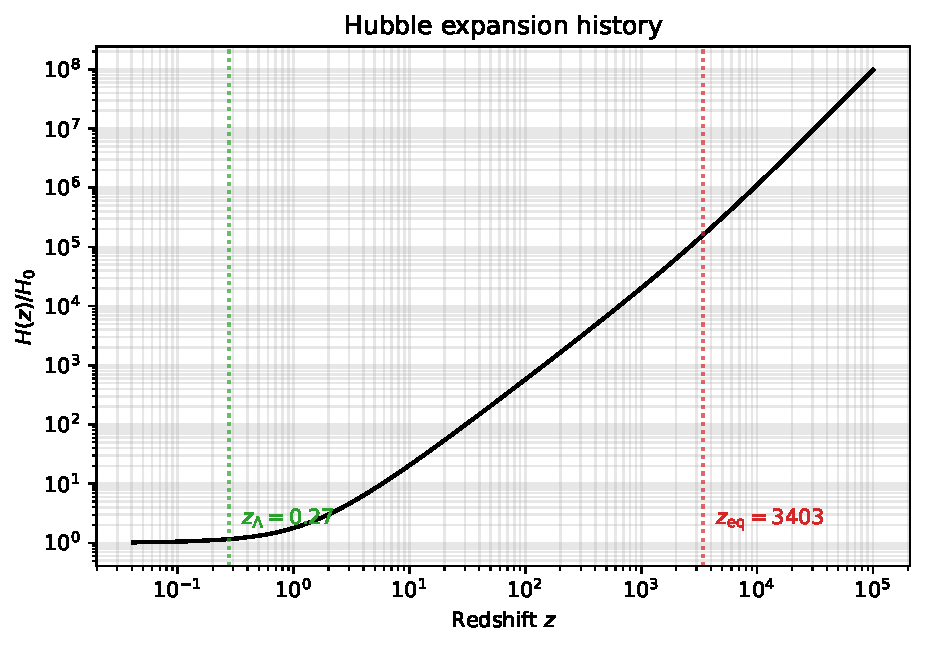
\includegraphics[width=0.85\linewidth]{figures/01_H_of_z.pdf}
\end{center}

\noindent The curve has three regimes. At $z \lesssim 0.3$, $H$ is nearly flat -- dark-energy domination. Between $z_\Lambda$ and $z_\mathrm{eq} \approx 3400$ matter dominates and $H \propto (1+z)^{3/2}$. Above $z_\mathrm{eq}$ radiation dominates and $H \propto (1+z)^2$. The change of slope at $z_\mathrm{eq}$ is subtle on a log-log plot but real -- it controls the relative heights of the CMB acoustic peaks (chapter 5).

\subsection{Plot: the composition of the universe}

The density fractions $\Omega_i(a) \equiv \rho_i(a)/\rho_\mathrm{tot}(a)$ make the era transitions visually explicit.

\begin{codebox}[Cell: plot $\Omega_i(a)$]
\begin{lstlisting}[style=python]
rho_r   = (bg['grhog'] + bg['grhornomass']) / a_grid**4
rho_m   = (bg['grhoc'] + bg['grhob']) / a_grid**3
rho_L   = bg['grhov'] * np.ones_like(a_grid)
rho_tot = rho_r + rho_m + rho_L

fig, ax = plt.subplots()
ax.loglog(a_grid, rho_m/rho_tot, label='Matter',    color='C0', lw=1.6)
ax.loglog(a_grid, rho_r/rho_tot, label='Radiation', color='C3', lw=1.6)
ax.loglog(a_grid, rho_L/rho_tot, label=r'$\Lambda$', color='C2', lw=1.6)
ax.axvline(bg['a_eq'], color='gray', ls=':', alpha=0.5)
ax.axvline(a_lambda,   color='gray', ls=':', alpha=0.5)
ax.text(bg['a_eq']*1.3, 1.2e-5, r'$a_\mathrm{eq}$', color='gray')
ax.text(a_lambda*1.3,   1.2e-5, r'$a_\Lambda$',     color='gray')
ax.set_xlabel('Scale factor $a$')
ax.set_ylabel(r'$\Omega_i(a)$')
ax.set_title('Composition of the universe')
ax.set_ylim(1e-6, 2); ax.set_xlim(1e-7, 1)
ax.legend(loc='lower right'); ax.grid(True, which='both', alpha=0.3)
plt.show()
\end{lstlisting}
\end{codebox}

\begin{center}
  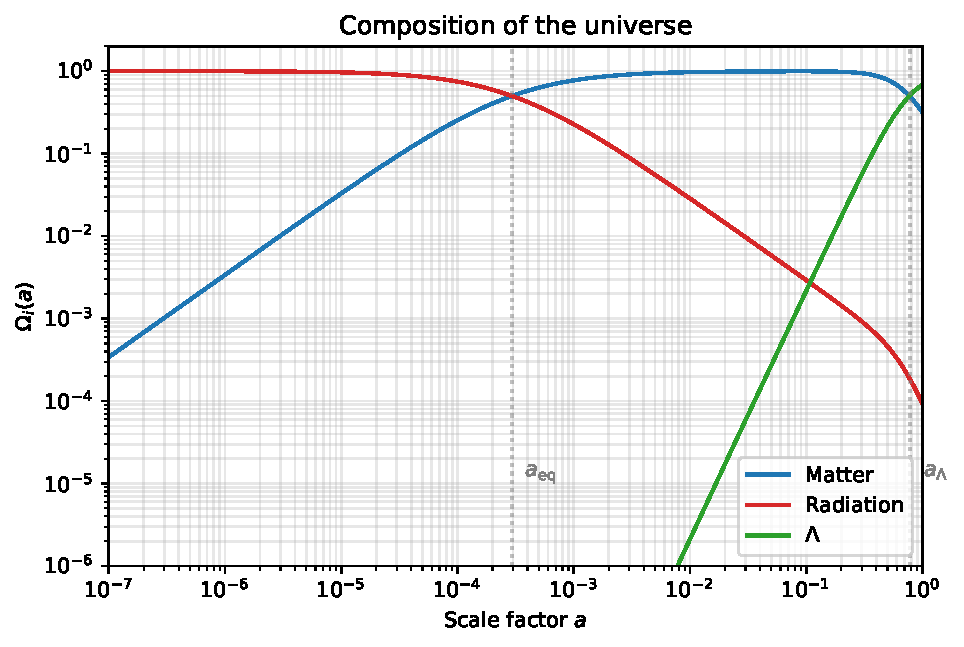
\includegraphics[width=0.85\linewidth]{figures/02_omega_of_a.pdf}
\end{center}

\noindent The radiation (red) and matter (blue) curves cross at $a_\mathrm{eq} \approx 3 \times 10^{-4}$, corresponding to $z_\mathrm{eq} \approx 3400$. The matter and $\Lambda$ curves cross at $a_\Lambda \approx 0.77$, corresponding to $z_\Lambda \approx 0.3$. Reading off $a = 1$: $\Omega_\Lambda \approx 0.69$, $\Omega_m \approx 0.31$, $\Omega_r \approx 9 \times 10^{-5}$.

\begin{physinsight}[The two horizons that matter for the CMB]
The CMB peak structure is set by two horizons:
\begin{itemize}
  \item the \emph{sound horizon at recombination} $r_s(\tau_*) \approx 147\,\mathrm{Mpc}$, the comoving distance a sound wave could have travelled before photons decoupled, which sets the acoustic peak spacing;
  \item the \emph{comoving distance to last scattering} $\chi_* \approx 14\,000\,\mathrm{Mpc}$, which projects the sound horizon to an angle $\theta_* = r_s/\chi_* \approx 0.6^\circ$ on the sky -- this is why the first acoustic peak is at $\ell \approx \pi/\theta_* \approx 220$.
\end{itemize}
Both are integrals over the background. Get $H(z)$ right and the peak locations come for free. By the end of this chapter your code can compute both of them.
\end{physinsight}

\subsection{Looking ahead}

The \texttt{bg} dictionary now contains everything chapter 2 needs to compute the recombination history: $H_0$, the densities of each species, the Thomson opacity prefactor \texttt{akthom}, the He/H number fraction \texttt{f\_He}, and the helper functions \texttt{total\_density\_a4}, \texttt{dtau\_da}, \texttt{hubble}, \texttt{conformal\_time}, \texttt{sound\_horizon}. Keep your notebook open. We will pick up directly from \texttt{bg}.
